\section{Problem Definition}
\label{sec:problem}

%The task of cross-lingual table linking: table info & entity info

%1. table info
%The task of cross-lingual table linking involves two kinds of information:
%mention tables and entities in the knowledge base.
The input mention table, denoted by $X$,
is a matrix of surface forms with $R$ rows and $C$ columns.
Each mention $x_{ij}$ is represented by a sequence of words
written in language $L_1$ (Chinese).
Given a knowledge base $K$ containing a set of entities $e$ written in language $L_2$ (English),
%The knowledge base, denoted by $K$, is made up of a finite set of unique entities $e$ written in language $L_2$, for example in English.
%Given the mention table $X$,
our task is to find the corresponding entity table $E$,
%such that for each position $(i, j) \in P$,
such that each entity $e_{ij} \in K$ correctly disambiguates the surface form $x_{ij}$. 
%\KZ{We don't need any info about the relations in the knowledge base?}

In practice, many mention tables contain unlinkable cells,
such as numbers, dates, times or emerging entities non-existent in the knowledge base.
There are some existing works that deal with the identification of
such numerical or temporal entities in web tables~\cite{ibrahim2016making}. 
In this paper, we will not focus on judging whether a cell is linkable or not.
Let $P$ denote a set of indices $(i, j)$
indicating the position of all linkable cells in a table,
and we assume that all linkable positions $P$ are provided along 
with the mention table $X$ in both training and testing datasets.

Traditional entity linking approaches
%\KQ{cites!}
usually formulate the task by defining a scoring function $S(x, e)$,
which measures the relevance between a mention $x$ and the target entity $e$.
Such techniques perform entity linking of each cell independently,
but the interaction between neighbourhood cells ignored in the scenario of table inputs.
To incorporate the coherence information between target entities in the table,
we define another scoring function for the table linking task, defined as follows:

\begin{equation}
  \label{eqn:joint-score}
  \hat{E} = \argmax_{E \in GEN(X)} S(X,E),
\end{equation}
\noindent
where $GEN(X)$ denotes the set of all candidate entity tables,
and the function measures the overall relevance score
between the whole input table and a candidate entity table.
%\KZ{This equation seems not useful: there's no info in there.I think this whole section can be cut. Just say a bit morein intro about the problem informally.}
%\begin{definition}
%\label{def:mention}
%A {\em mention table} $T_M$ is a tuple $(\textbf{m}, P, L_1)$, where:
%$\textbf{m}$ is a matrix of mentions and $\textbf{m}_{ij}$ represents a specific cell in table at $i^{th}$ row and $j^{th}$ column;
%$P$ is a set of indices $\langle i,j  \rangle$ indicating $\underline{P}$osition of cells needs to be linked;
%$L_1$ is the language in which table mentions $\textbf{m}$ are written.
%\end{definition}
%
%\begin{definition}
%	A {\em Knowledge Base} $K$ is a tuple $(E, L_2)$, where:
%	$E$ is a finite set of unique entities in $KB$;
%	$L_2$ is the language in which $KB$ is written.
%\end{definition}
%
%\begin{definition}
%An {\em entity table} $T_E$ is a tuple $(\textbf{e}, P, L_2)$, where:
%$\textbf{e}$ is a matrix of entities and $\textbf{e}_{ij} \in E$ represents a specific cell in table at $i^{th}$ row and $j^{th}$ column;
%$P$ is a set of indices $\langle i,j  \rangle$ indicating $\underline{P}$osition of cells have been linked;
%$L_2$ is the language in which linked entities $\textbf{e}$ are written.
%\end{definition}
%
%\begin{definition}
%Cross-lingual table linking seeks to find a mapping $\mathcal{F}$ between a mention table $T_M$ and an entity table $T_E$, so that each mention $\textbf{m}_{ij}$ where $\langle i,j\rangle \in M$ is linked to a corresponding entity $\textbf{e}_{ij}$.
%\end{definition}
%

%In this paper, we assume that all the web tables have been preprocessed to 
%remove all unlinkable columns (or rows), and as a result, every cell in the input table can be linked, unless the knowledge base doesn't contain the corresponding entity, which is shown as grey cell in \figref{fig:problem}. All the red cells in mention table will be linked to corresponding purple cells in entity table.
%
% 
%\begin{figure}[th]
%	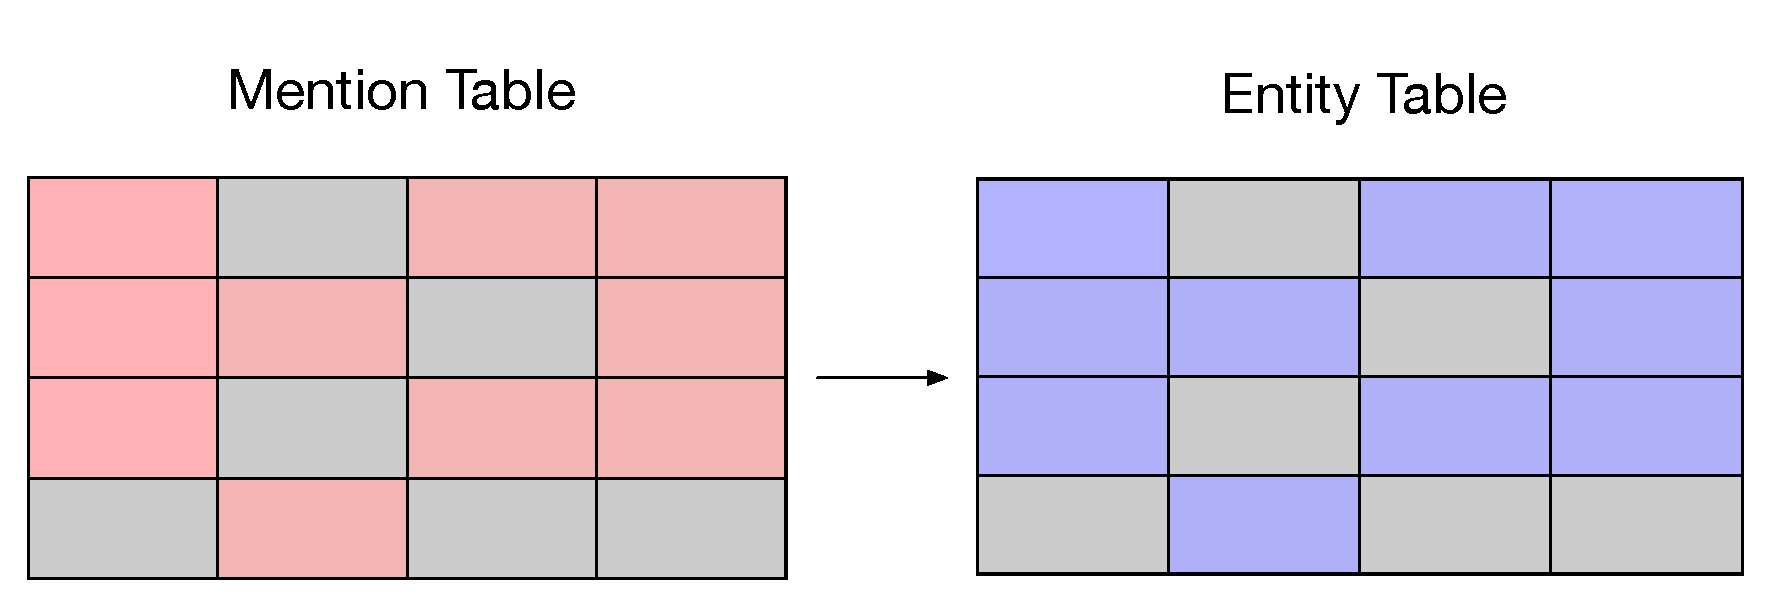
\epsfig{file=figures/problem.eps, angle=0, width=1.0\columnwidth}
%	\caption{Snapshot of cross-lingual table linking}
%	\label{fig:problem}
%\end{figure}
%
